\chapter[Efecto de la concentraci\'on osm\'otica y temperatura en la imbibici\'on y germinaci\'on de semillas de papaya]{Germinaci\'on}

\begin{Huge}
	\begin{center}
		\textbf{Determinar la imbibici\'on y germinaci\'on de semillas de papaya en diferentes temperaturas y condiciones osm\'oticas}
	\end{center}
\end{Huge}

\section{Introducci\'on}

La semilla es una estructura que se desarrolla a partir del ovulo despu\'es de la fertilizaci\'on. Est\'a constituido por un embri\'on, el tejido que almacena los nutrientes, y las cubiertas seminales. Las semillas de las angiospermas est\'an contenidas dentro del fruto que se desarrolla de las paredes del ovario, sin embargo, en las plantas gimnospermas la semilla est\'a expuesta y no se encuentra dentro del fruto.

Cabe resaltar que la semillas se encuentran extremadamente deshidratadas, en consecuencia las reacciones metab\'olicas son escasamente detectables. Est\'a caracter\'istica permite al embri\'on sobrevivir en condiciones adversas por largos periodos de tiempo. La semilla, por tanto, est\'a en una fase quiescente\footnote{La definici\'on de la RAE es que est\'a quieto pudiendo tener movimiento propio} y representa una etapa normal en el ciclo de vida de una planta. 

La germinaci\'on es la reanudaci\'on del crecimiento del embri\'on. En condiciones de campo, la tasa de germinaci\'on puede ser controlada por el potencial h\'idrico del suelo y la temperatura. El potencial h\'idrico del suelo es la suma del potencial m\'atrico y el componente de solutos solubles que posee. Con respecto a la temperatura est\'a depende de la especie, por lo tanto, el rango de temperatura determina el h\'abitat y la distribuci\'on geogr\'afica en las plantas.

El proceso de germinaci\'on da inicio cuando la semilla absorbe agua y dicho proceso se le conoce como imbibici\'on. La rehidrataci\'on de los tejidos de la semilla es llevada a cabo por fuerzas matricas que son el resultado de la atracción química y electrostática del agua hacia las paredes celulares y materiales celulares hidrof\'ilicos. En consecuencia, la semilla se hincha causando una ruptura de las cubiertas seminales permitiendo al embri\'on emerger \citep{hopkins2009introduction}. 

\begin{table}[h]
	\caption{Intervalo de Temperaturas optimas, m\'aximas, media, y potencial h\'idrico para la germinaci\'on de semillas de plantas de cultivo.}
	\label{tabla:germinacion}
	\begin{tabular}{p{0.17\textwidth}p{0.17\textwidth}p{0.17\textwidth}p{0.17\textwidth}p{0.17\textwidth}}
		\hline
		Cultivo & T$_{opt}$ & T$_{50\%}$ & T$max$  & $\Psi$ \\ % Topt , Tb50% germ, Tmax 
		\hline
		Trigo &   & 1.2-1.6 & 30 & -2.9 \\
		
		Arroz & 30 & 10 &  &  \\

		Ma\'iz & 32 & 8-8.2  &   & -1.6 \\

		Sorgo & 35.8 & 11 & 45 &  \\
		
		Algod\'on & 33-36 & 14 & 40  & -1 \\
		
		Soya & 34 & 4-10 & 40-50 &  \\
		
		Frijoles & 32 & 6.6 & 48 & -2.3 \\
		\hline
		\multicolumn{5}{l}{\footnotesize Valores obtenidos de \citet{drr2014lrag}}
	\end{tabular}
\end{table}

Con respecto a la temperatura, puede influenciar la tasa de imbibici\'on y en consecuencia el proceso de germinaci\'on. En el cuadro \ref{tabla:germinacion} se presentan las temperaturas optimas para la germinaci\'on, as\'i como los valores m\'aximos. 

\section{Principio}

El agua en diferentes concentraciones osm\'oticas puede causar un estr\'es salino. Por lo tanto, puede afectar los procesos de imbibici\'on y germinaci\'on de la semilla al disminuir el potencial h\'idrico del agua. 

% Fundamentos de fisiolog\'ia pagina 563

% Hopkins Introduction to plant physiology pag 301

% Plant physilogy Sinauer Associates

\section{Objetivo general}

Evaluar el efecto de diferentes concentraciones osm\'oticas en la imbibici\'on y germinabilidad de las semillas de papaya en diferentes temperaturas. 

\section{Obejetivo espec\'ifico}

\begin{enumerate}
	\item Determinar el porcentaje de imbibici\'on de semillas de papaya \textit{Carica papaya} en soluciones de 0.5 y 1.0M de $NaCL$ en temperatura ambiente y baja temperatura (4-5 $^\circ$C).
	\item Determinar el porcentaje de germinaci\'on de semillas de papaya \textit{Carica papaya} en soluciones de 0.5 y 1.0M de $NaCL$ en temperatura ambiente y baja temperatura (4-5 $^\circ$C).
\end{enumerate}

\section{Materiales}

\subsection{Material requerido }

\begin{enumerate}
	\item 18 platos petri o vasos de pl\'astico
	\item Matraz aforado de 1 L
	\item Agua destilada
	\item 100g $NaCL$
	\item Semillas de papaya
\end{enumerate}

\subsection{Material por grupo}

\begin{enumerate}
	\item Balanza anal\'itica
	\item Papel secante
\end{enumerate}

\section{Metodolog\'ia}

\subsection{Preparaci\'on de reactivos}

Para preparar la soluci\'on de 0.5 y 1.0M de $NaCl$ se disuelve 29.25 y 58.5g de $NaCl$ en un litro de agua destilada, respectivamente. 

\subsection{Procedimiento}  

Conseguir semillas en un vivero o centro autorizado. Tambi\'en se puede ocupar las que se encuentran dentro del fruto, si eliges est\'a opci\'on tienes que lavar muy bien la semilla para que no tenga ning\'un residuo org\'anico. Una forma muy sencilla de seleccionar semillas viables es dejarlas en un recipiente con agua por 10 minutos y desechar las semillas que flotan. Luego se procede a desinfectar las semillas, por tanto, debes sumergirlas en agua, agregar cuatro gotas de cloro y esperar cinco minutos. Posteriormente, se enjuagan bien con agua destilada o con agua de garraf\'on unas tres o cuatro veces. 

\begin{figure}[h]
	
	\begin{leftbar}
		
		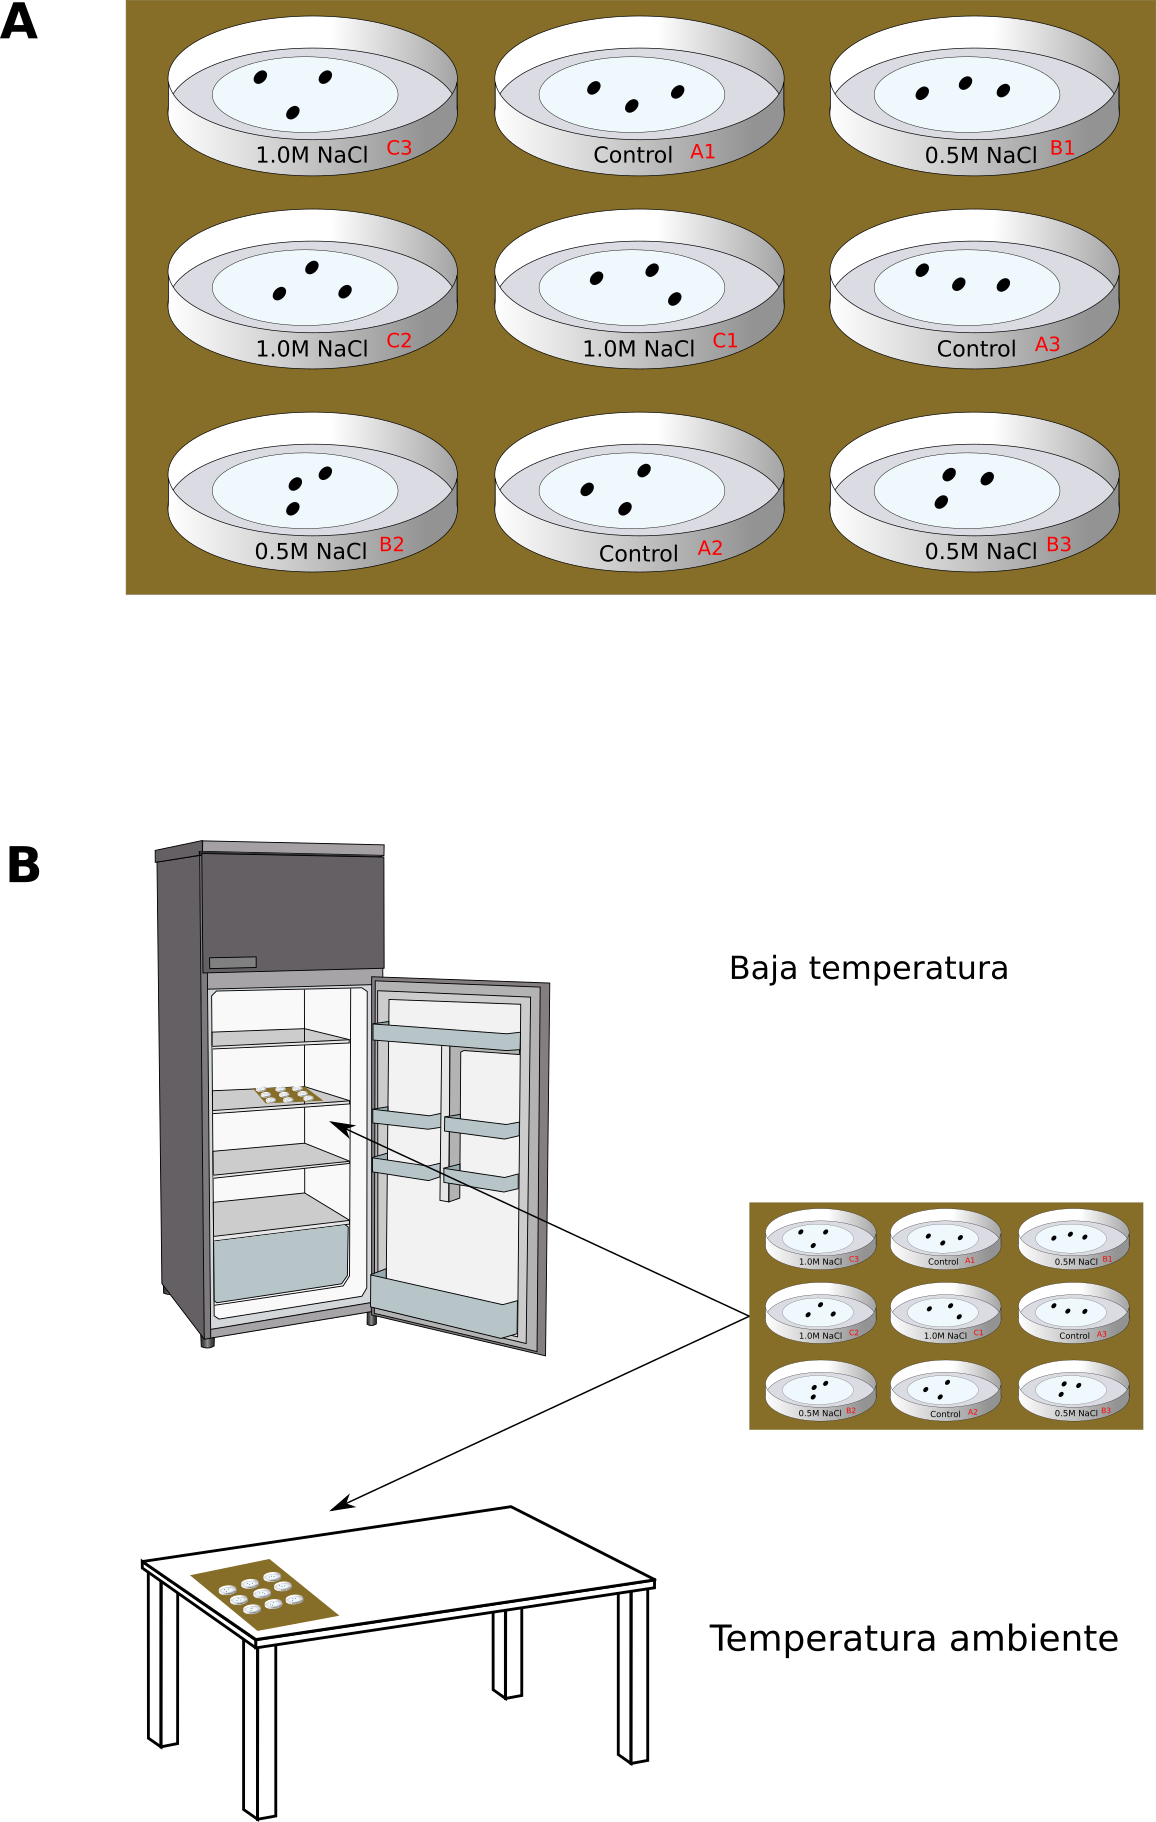
\includegraphics[width=0.5\textwidth]{Petri2.png}
		\centering
		\caption{\textit{\textbf{A}: colocaci\'on aleatoria de los tratamientos para la determinaci\'on del porcentaje de imbibici\'on y germinaci\'on en soluciones de 0.5, 1.0M de NaCl, y agua destilada como control. \textbf{B}: tratamientos condici\'on de temperatura ambiente y baja temperatura.}}
		\label{fig:petri}
		
	\end{leftbar}
	
\end{figure}

A continuaci\'on se forman nueve grupos de semillas por condici\'on de temperatura, cada grupo puede tener entre tres a cuatro semillas. Se registra el peso inicial de cada semilla. Luego se coloca un grupo de semilla en cada plato petri (o en vaso de pl\'astico desechable) sobre papel absorbente (Figura \ref{fig:petri}). Posteriormente, se agrega el mismo volumen de soluci\'on con una jeringa de 5 mL y se cubre el plato petri. Los tratamientos consisten en un control con agua destilada (o de garraf\'on), soluciones de 0.5 y 1.0M de NaCl, por triplicado cada tratamiento. 

Despu\'es de dos o cuatro d\'ias se vuelve a registrar el peso de las semillas, y el n\'umero de semillas germinadas. Por lo tanto, se calcula el porcentaje de imbibici\'on y germinaci\'on, respectivamente.

$$\text{Imbibici\'on} (\%) = \frac{P_2 - P_1}{P_1} \times 100$$ 

Donde:

\begin{itemize}
	\item $P_1 =$ peso inicial del lote de semillas (en cada plato petri).
	\item $P_2 =$ peso del lote de semillas, despu\'es del tiempo indicado.
\end{itemize}

$$\text{Germinaci\'on} (\%) = \frac{SG}{TS} \times 100$$

Donde:

\begin{itemize}
	\item $SG =$ n\'umero de semillas germinadas.
	\item $TS =$ n\'umero total de semillas. 
\end{itemize}

Tome en cuenta las siguientes precauciones: seleccionar semillas sanas, evitar contaminaci\'on y el tratamiento a temperatura ambiente debe estar en un lugar seco y con sombra. Las muestras deben mantenerse h\'umedas durante el tiempo del experimento, por lo tanto, deben de taparse bien. 

\section{Resultados}

Los resultados obtenidos se pueden presentar en el cuadro \ref{resultados:germinacion}.

\begin{table}[h!]
	\caption{Datos de porcentaje de imbibici\'on y germinaci\'on de semillas de papaya en diferentes concentraciones de $NaCl$ y temperaturas de incubaci\'on.}
	
	\label{resultados:germinacion}
	\centering
	\begin{tabular}{p{0.17\textwidth} p{0.17\textwidth} p{0.17\textwidth} p{0.17\textwidth} p{0.17\textwidth}}
		
		\hline  &&&& \\
		Temperatura & Soluci\'on (M) & Repetici\'on & Imbibici\'on (\%) & Germinaci\'on (\%) \\
		\hline 
		
		\multirow{9}{*}{Ambiente}& \multirow{3}{*}{Control} & A1 & & \\ 
															%\cline{3-5}
														   & & A2 & & \\
														   %\cline{3-5}
														   & & A3 & & \\
														   \cline{2-5}
														   
								 & \multirow{3}{*}{0.5}		 & B1 & & \\
															 &&B2&& \\
															 &&B3&& \\
															\cline{2-5} 
		 &\multirow{3}{*}{1.0}& C1 && \\
		&&C2&& \\
		 &&C3&& \\
		
		\hline 
		\multirow{9}{*}{4-5 $^\circ$C}& \multirow{3}{*}{Control} & A1 & & \\ 
		& & A2 & & \\
		& & A3 & & \\
		\cline{2-5} 
		& \multirow{3}{*}{0.5}		 & B1 & & \\
		&&B2&& \\
		&&B3&& \\
		\cline{2-5} 
		&\multirow{3}{*}{1.0}& C1 && \\
		&&C2&& \\
		&&C3&& \\
		
		\hline 
					
	\end{tabular}
\end{table}



\section{Cuestionario}

\begin{enumerate}
	\item \textquestiondown C\'omo explica la relaci\'on entre la concentraci\'on osm\'otica y el porcentaje de imbibici\'on?
	\item \textquestiondown Por qu\'e influy\'o la temperatura en el porcentaje de germinaci\'on?
	
\end{enumerate}
